\subsection{Administração global de servidores}

Na seção anterior, ao debatermos a crise de remoção do modo emergencial do captcha na Wikipédia em português foi citada ``a comunidade de técnicos que mantém os servidores'' do movimento Wikimedia, e aqui iremos versar um pouco mais sobre ela.

Apesar de descentralizado política e editorialmente, o movimento Wikimedia é bastante centralizado quando observada sua infraestrutura tecnológica. \citewiki{enwiki_wikimedia_servers} Editores interessados em iniciar uma enciclopédia em um novo idioma não precisam entender nada sobre programação ou manutenção de servidores. Uma vez aprovada, sua nova wiki será criada dentro da \textit{wikifarm} \footnote{Termo em inglês que em tradução literal seria uma ``fazenda de wikis'', que se refere a um conjunto de instalações do MediaWiki que compartilham recursos, configurações e ferramentas administrativas.} na nuvem do movimento Wikimedia, e será mantida por esta comunidade global de administradores de sistemas.

\begin{figure}
    \centering
    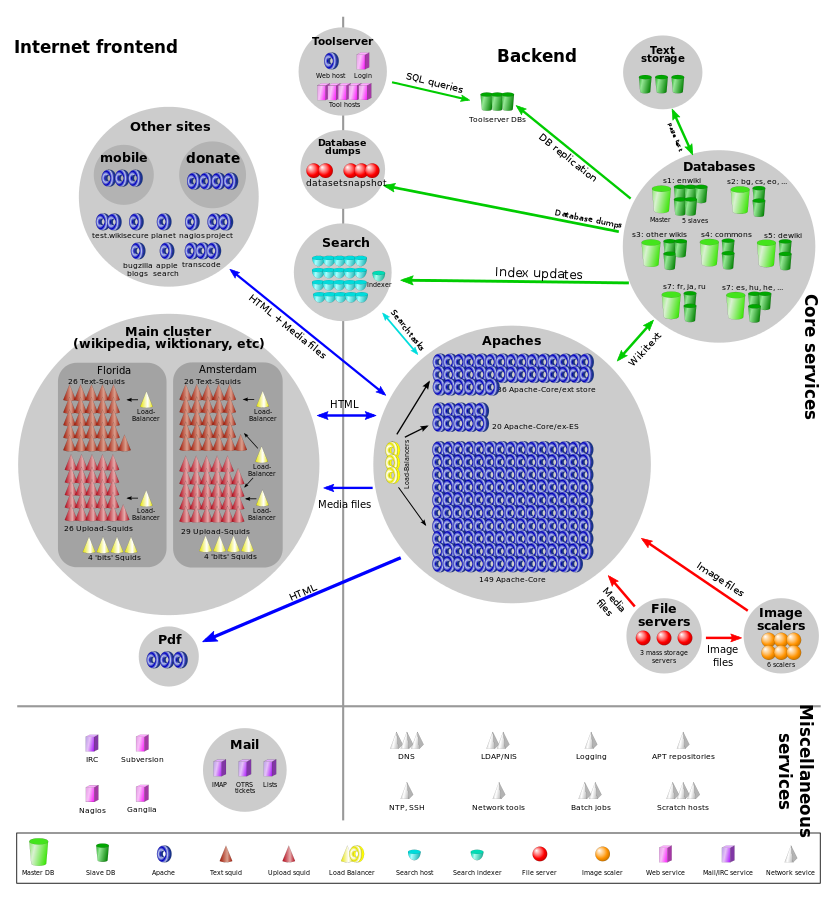
\includegraphics[width=1\textwidth]{Images/servidores_movimento_wikimedia.png}
    \caption{Estrutura dos servidores do Movimento Wikimedia. \citewiki{enwiki_wikimedia_servers_svg}}
    \label{fig:servidores_movimento_wikimedia}
\end{figure}

Os administradores de sistema do Movimento Wikimedia são divididos em três níveis de acesso com permissões distintas: ``\textit{Ops}'', que tem pleno acesso às máquinas da nuvem. ``\textit{Deployment}'', que permite alterar alguns códigos-fonte que rodam nos servidores, e ``\textit{Restricted}'', que podem executar alguns scripts de manutenção e ler os logs dos servidores.

Em setembro de 2020 existem 31 usuários com permissão completa (``\textit{ops}''),  11 com ``\textit{restricted}'' e 55 com acesso de ``\textit{Deployment}''. Dos 31 com acesso pleno, hoje apenas 1 único usuário, ``Ori Livneh'', é voluntário. Todos os outros são funcionários da WMF. Dentre os ``restricted'', novamente encontramos apenas um voluntário em meio a funcionários da fundação, e na categoria ``Deployment'' meia dúzia deles, alguns poucos funcionários da WMDE \footnote{Capítulo alemão do movimento Wikimedia. Estrutura a ser explicada na próxima seção} e dezenas de funcionários da WMF. \citewiki{enwiki_wikimedia_system_administrators}

Esse cenário nos mostra que esta hoje não é uma comunidade como as demais do movimento Wikimedia, compostas em sua vasta maioria por voluntários. Aqui estes são a exceção, e o fato da WMF ser a empregadora de praticamente todos os membros, na prática a coloca em um local de dona das decisões tomadas.

Muitos não veem problemas nesta concentração de poder em um ponto central do movimento, pois as tarefas realizadas por esta comunidade afinal são ``meramente técnicas'' e assim sua composição seria irrelevante, tal como em um ``mito da universalidade e da neutralidade da Ciência pura''. Mito este que segundo Ivan da Costa Marques, ``\textit{prega que o conhecimento científico independe de quem o produziu. Não interessa se o cientista é branco ou negro, mestiço, rico ou pobre, gay, homem, mulher, judeu, muçulmano ou católico, em que século ou região vive ou sob que regime político trabalha, pois a verdade ou o fato científico transcende as contingências locais e sociais e paira acima delas}'' (\cite[p.13]{marques_2005}).

Assim, para o movimento Wikimedia, deve caber aos técnicos ``apenas'' implementar as questões que forem decidas pelas demais comunidades de forma neutra e imparcial, não sendo facultada a esta comunidade a liberdade de ``fazer política''.

Porém, na prática, esta comunidade atua como a principal interface entre os usuários humanos do movimento e os servidores onde são rodados os softwares. Tal como um tribunal superior, está em suas mãos o poder de fazer ou não o que lhe convir, e quando lhe interessar.

Como vimos na seção anterior sobre a crise do captcha, se esta comunidade (ou a WMF, que quase pode ser utilizada como sinônimo aqui pelo alinhamento de interesses) decide que uma decisão local fere os valores do movimento, ela pode simplesmente se negar a implementar a decisão tomada, ou até mesmo se utilizar de meios para reverter alterações que possam ter sido realizadas localmente. Assim como, de forma dura (e que alguns diriam inclusive ditatorial), pode tomar decisões que alterem dinâmicas de funcionamento local e até mesmo encerrem comunidades.

Foi isso o que aconteceu com a Wikipédia em Klingon, em agosto de 2005. Jimbo Wales, um dos fundadores da Wikipédia e o primeiro usuário com permissão ``ops'' nos servidores, fez uma solicitação que fora prontamente atendida por outro ``op'', Brion Vibber, bloquando esta Wikipédia para edição. Brion informou sua ação em um curto e-mail enviando para a lista wikimedia-l: ``\textit{Eu travei a Wikipédia em Klingon (tlh.wikipedia.org) a pedido de Jimmy. Ela continua online por hora, mas não é mais editável}''. \footnote{Tradução livre do original em inglês: ``\textit{I've locked the Klingon Wikipedia (tlh.wikipedia.org) on Jimmy's request. It remains online for now, but is no longer editable.}'' \citewiki{enwiki_wikimedia_klingon_locked}}

Na página do movimento que conta a história da Wikipédia em Klingon podemos ler que Wales ``\textit{nunca declarou publicamente seus motivos para fechar a wiki}'' \footnote{Tradução livre do original em inglês: ``\textit{Jimbo has never publicly stated his exact rationale for closing the wiki}'' \citewiki{enwiki_wikimedia_klingon_history}}, e somos informados de que seu conteúdo, que estava em licença livre, fora migrado para outro servidor de wikis, fora do movimento Wikimedia.

Destino similar teve a Wikipédia em Toki Pona. Como nos conta Bialous (\citeyear[p.171]{bialous_sztuczne_2017}) , ``\textit{as versões em Klingon e Toki Pona da Wikipédia foram retiradas deste site e transferidas para o Fandom, um site de cultura de fãs que também oferece a possibilidade de coletar artigos enciclopédicos no estilo da Wikipédia.}'' \footnote{Tradução com apoio do Google Translate do original em polonês: ``\textit{Wersje Wikipedii w językach klingońskimoraz toki pona zostały wycofane z tego serwisu i przeniesione na Fandom,portal dla kultur fanowskich, dający również możliwość gromadzenia arty-kułów encyklopedycznych na wzór Wikipedii.}}'' Ainda segundo Bialous (\citeyear[p.171]{bialous_sztuczne_2017}), ambas as wikis não contavam com mais de 500 verbetes cada quando foram encerradas no ecossistema da Wikipédia, e talvez pela baixa representatividade de suas comunidades tenha sido tomada a decisão de cima para baixo de encerrá-las.

Em uma rápida consulta aos bancos de dados públicos do movimento, encontramos 11 diferentes Wikipédias que já foram fechadas nesta \textit{wikifarm} (\cite{quarry_close_wikipedias}), que se somam a quatro outras que haviam sido removidas anteriormente ao estabelecimento desta arquitetura de servidores que mantém o registro das wikis desativadas \citewiki{enwiki_wikimedia_list_wikipedias}, totalizando 15 comunidades wikipedistas que foram encerradas pelo movimento global.

O caso das Wikipédias fechadas pode parecer um tanto quanto dramático e extremo, mas serve para ilustrar até qual medida vai o poder daqueles que detém as senhas administrativas dos servidores do movimento. E, como observado por Feitosa (\cite[p.5]{latour_cogitamus_2010} apud), ``\textit{independentemente da intencionalidade ou do controle que o construtor tenha objetivado, sua obra continuará 'oferecendo permissões, possibilidades, concessões', ainda que não previstas ou desejadas, ou seja, continuará fazendo algum tipo de política}''. Assim, na próxima seção iremos explorar mais detalhadamente este modelo de governança global-local do movimento Wikimedia, e daremos mais exemplos desta ``agência política'' da comunidade ``meramente técnica''.